\chapter{Experimental Setup}
\label{chap:experimental_setup}

This chapter defines the reproducibility contract for the empirical analysis:
dataset splits, model architecture, attack suite, training configuration,
hyperparameters, statistical protocol, evaluation metrics, graybox transfer
design, and experiment tracking. Results and interpretation are reserved for
Chapter~\ref{chap:results_analysis}.

\section{Dataset and Preprocessing}

The experiments are conducted on CIFAR-10~\cite{krizhevsky2009learning}, a standard image-classification benchmark consisting of ten object categories. 

\begin{figure}[H]
\centering
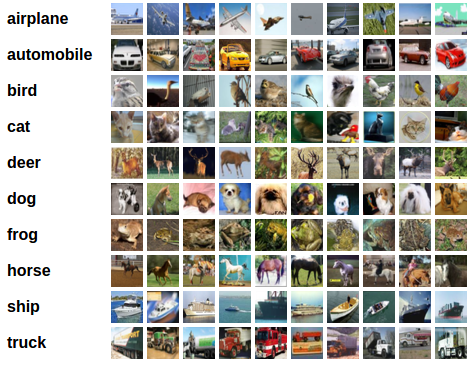
\includegraphics[width=0.72\linewidth]{figures/cifar10.png}
\caption[CIFAR-10 example images]{Example images from the CIFAR-10 dataset. CIFAR-10 contains ten object categories represented by low-resolution \(32 \times 32\) color images.}
\label{fig:ch5_cifar10_examples}
\end{figure}
Each image has spatial resolution \(32 \times 32\) with three color channels. The official dataset contains 50,000 training images and 10,000 test images. In our experimental pipeline, the original training split is partitioned into 40,000 images for training and 10,000 images for validation and checkpoint selection, while the official 10,000-image test split is reserved for final test-set evaluation.

The validation set is used only for model selection and hyperparameter monitoring. Final reported numbers are computed on the test set after the checkpoint has been selected. This separation is important because adversarial robustness estimates can vary across random seeds and training checkpoints; using a held-out validation set reduces the risk of selecting a checkpoint based on test-set performance.
All images are normalized using the same preprocessing pipeline across methods. During training, standard CIFAR-10 data augmentation is applied to the clean images before adversarial examples are generated. The augmentation includes random cropping with padding and random horizontal flipping. During validation and testing, no stochastic augmentation is used. This ensures that differences between methods are caused by the training objective rather than by differences in preprocessing or evaluation.

The same dataset split, preprocessing pipeline, and evaluation dataloaders are used for all compared methods. This includes the single-attack PGD-AT and DDN-AT baselines, Multi-AT, AttackDRO, Cluster-DRO, and AttackDRO++.

\section{Model Architecture}

The primary architecture used in this study is ResNet-18, based on the residual learning
framework of He et al.~\cite{he2016deep}, adapted for CIFAR-10 resolution. ResNet-18
provides a useful balance between expressiveness and computational cost: it is large
enough to support nontrivial adversarial training experiments, but still efficient enough
to run repeated-seed comparisons and ablation studies.

The classifier is denoted by \(f_\theta\). For an input image \(x\), the model outputs logits
$$
z = f_\theta(x) \in \mathbb{R}^{C},
$$
where \(C=10\) is the number of CIFAR-10 classes. In addition to logits, the proposed method requires access to the penultimate-layer representation
$$
h = \phi_\theta(x) \in \mathbb{R}^{d_h}.
$$

This feature vector is used for clustering adversarial examples in AttackDRO++ and for constructing the gradient-fingerprint augmented feature described in Chapter 4. For ResNet-18 on CIFAR-10, the penultimate representation dimension is \(d_h = 512\). Therefore, the raw classifier-head gradient proxy has dimension \(C d_h = 10 \times 512 = 5120\), which is later reduced by random projection.

Unless otherwise stated, all main experiments use the same ResNet-18 architecture and differ only in the training objective. This controlled setup ensures that performance differences can be attributed to the training method rather than to architectural changes. Higher-capacity architectures are treated as scaling checks or future extensions rather than the main basis for comparison.

\section{Attack Suite and Configuration}
% TODO[Kiệt]:
% Goal:
% - Make this section the source of truth for attack names and configurations.
% Flow:
% - Separate source/training attacks from evaluation-only attacks and AutoAttack.
% - Define PGD-$\ell_\infty$ once as the 20-step cross-entropy source attack.
% Include:
% - Ensure tables cover attack, norm, budget, steps, loss/objective, role, and whether used for training/evaluation.
% - Cite docs/05_notation_registry.md names in formal table/caption text.
% Avoid:
% - Repeating code-style names like `PGD20-CE` in prose.
% Target length: 4-6 paragraphs plus configuration tables.
Stage 2 evaluates whether robustness learned from a small set of source attacks generalizes to a broader attack suite. The attack suite is divided into two groups: source attacks used during training and evaluation attacks used only for validation or final testing.

\subsection{Training attacks}
The main training setup uses two source attacks:
\[
    \mathcal{A}_{\mathrm{src}}
    =
    \{\text{PGD-}\ell_\infty,\text{DDN-}\ell_2\}.
\]
PGD-\(\ell_\infty\) represents the standard first-order \(\ell_\infty\) adversarial
training setting. It uses cross-entropy loss and perturbation budget
\(\varepsilon_\infty = 8/255\). DDN-\(\ell_2\) is based on the Decoupled Direction and
Norm attack of Rony et al.~\cite{rony2019decoupling}. DDN is an efficient gradient-based
\(\ell_2\) attack that decouples the perturbation direction from its norm: the direction
is updated using gradient information, while the perturbation norm is adapted depending
on whether the current example is already adversarial.



Table~\ref{tab:training_attacks} summarizes the source attacks used during training.
Both attacks are used to generate mixed adversarial minibatches for Multi-ATtack
ERM, AttackDRO, AttackDRO++, and the proposed AttackDRO++ Anchor35 GradFP method.

\begin{table}[H]
\centering
\caption{Training attack configuration.}
\label{tab:training_attacks}
\begin{tabular}{llllll}
\toprule
Attack & Norm & Budget & Steps & Loss / objective & Role \\
\midrule
PGD-{$\ell_\infty$} & $\ell_\infty$ & $8/255$ & 20 & Cross-entropy & Source attack \\
DDN-$\ell_2$ & $\ell_2$ & $0.5$ & 20 & DDN objective & Source attack \\
\bottomrule
\end{tabular}
\end{table}

ForMulti-ATtack training, each minibatch is split across the source attacks and adversarial examples are generated using the assigned attack. The same mixed-batch source attack construction is also used by AttackDRO, AttackDRO++, and the proposed AttackDRO++ Anchor35 GradFP method. Thus, the compared methods share the same adversarial data generation process and differ mainly in how they weight or group the generated examples.

\subsection{Evaluation Attacks}
\label{sec:evaluation_attacks}

The evaluation suite includes both source attacks and held-out attacks. The two source
attacks used during training are also included in validation and test evaluation, while
the remaining attacks are held out from training. This protocol directly tests the
attacks-as-domains hypothesis: a robust model should not only perform well on the attacks
used for optimization, but should also generalize to attacks with different perturbation
geometries and optimization dynamics.


For validation and final testing, we evaluate each checkpoint using the attack suite in
Table~\ref{tab:evaluation_attacks}. The main aggregate metric, denoted Mean(8), is
computed over the eight attacks in the table. AutoAttack is reported separately and is
therefore not included in Mean(8).
\begin{table}[H]
\centering
\caption{Validation and test attacks used for Mean(8).}
\label{tab:evaluation_attacks}
\renewcommand{\arraystretch}{1.08}
\setlength{\tabcolsep}{7pt}
\begin{tabular}{lcccc}
\toprule
Attack & Norm & Budget & Steps & Group \\
\midrule
FGSM-RS              & $\ell_\infty$ & $8/255$ & 1   & Held-out $\ell_\infty$ \\
PGD-$\ell_\infty$   & $\ell_\infty$ & $8/255$ & 20  & Source \\
TPGD                 & $\ell_\infty$ & $8/255$ & 10  & Held-out $\ell_\infty$ \\
MI-FGSM              & $\ell_\infty$ & $8/255$ & 10  & Held-out $\ell_\infty$ \\
PGD-$\ell_2$         & $\ell_2$      & $0.5$   & 10  & Held-out $\ell_2$ \\
DDN-$\ell_2$         & $\ell_2$      & $0.5$   & 20  & Source \\
DeepFool-$\ell_2$    & $\ell_2$      & $0.5$   & 50  & Held-out $\ell_2$ \\
CW-$\ell_2$          & $\ell_2$      & $0.5$   & 200 & Held-out $\ell_2$ \\
\bottomrule
\end{tabular}
\end{table}

For aggregate analysis, we report four summary metrics derived from the same eight
attacks: Seen, Held-out \(\ell_\infty\), Held-out \(\ell_2\), and Mean(8). Their exact
definitions are given in Section~\ref{sec:evaluation_metrics}.

\paragraph{AutoAttack configuration}

AutoAttack is used as an additional standardized \(\ell_\infty\) stress test following
Croce and Hein~\cite{croce2020reliable}. It is not included in Mean(8), because it is
computationally more expensive and follows a separate evaluation protocol.

The AutoAttack configuration uses the standard \(\ell_\infty\) setting with perturbation
budget \(\varepsilon_\infty = 8/255\). In early experiments and ablations, AutoAttack is
sometimes evaluated on a subset of 512 test samples as a sanity check. These 512-sample
results are useful for detecting severe robustness collapse, but they are not used as the
primary ranking criterion because the sample size is smaller and the variance is higher.
For the final stress test, AutoAttack is evaluated on the full test set for selected
representative seeds.

\begin{table}[H]
\centering
\caption{AutoAttack configuration.}
\label{tab:autoattack_config}
\renewcommand{\arraystretch}{1.08}
\setlength{\tabcolsep}{10pt}
\begin{tabular}{lccc}
\toprule
Attack & Norm & Budget & Role \\
\midrule
AutoAttack & $\ell_\infty$ & $8/255$ & Separate stress test \\
\bottomrule
\end{tabular}
\end{table}

\section{Training Configuration}

All methods are trained under a controlled adversarial training pipeline. Unless
otherwise stated, the optimizer, model architecture, dataset split, preprocessing
pipeline, and evaluation protocol are kept fixed across methods. This ensures that
performance differences mainly come from the training objective rather than from
implementation or evaluation differences.

To make method differences attributable to the training objective, Table~\ref{tab:ch5_training_config}
fixes the shared training configuration for the main experiments. All main experiments use ResNet-18 on CIFAR-10 with stochastic gradient descent (SGD),
momentum, weight decay, mixed-precision training, and a multi-step learning-rate
schedule. The main methods are trained for 50 epochs. During training, each minibatch
contains a balanced mixture of source attacks. In the two-source setting, approximately
half of the minibatch is assigned to PGD-\(\ell_\infty\) and the other half to
DDN-\(\ell_2\).

\begin{table}[H]
\centering
\caption{General training configuration used for the main experiments.}
\label{tab:ch5_training_config}
\footnotesize
\setlength{\tabcolsep}{4pt}
\renewcommand{\arraystretch}{1.08}
\begin{tabularx}{\textwidth}{@{}
>{\raggedright\arraybackslash}p{0.25\textwidth}
>{\raggedright\arraybackslash}p{0.22\textwidth}
>{\raggedright\arraybackslash}X
@{}}
\toprule
Component & Setting & Description \\
\midrule
Dataset & CIFAR-10 & 40k train / 10k validation / 10k test. \\
Backbone & ResNet-18 & CIFAR-10 adapted residual network. \\
Training epochs & 50 & Main training budget. \\
Batch size & 128 & Used for all main methods. \\
Optimizer & SGD & Momentum-based stochastic gradient descent. \\
Momentum & 0.9 & Standard SGD momentum. \\
Weight decay & $5 \times 10^{-4}$ & Weight regularization. \\
Initial learning rate & 0.1 & Decayed during training. \\
Learning-rate schedule & Multi-step & Same schedule for all compared methods. \\
Mixed precision & Enabled & Reduces memory usage and training time. \\
Gradient clipping & Enabled & Stabilizes adversarial training. \\
Checkpoint selection & Validation robust average & Test set is used only after selection. \\
\bottomrule
\end{tabularx}
\end{table}

Checkpoint selection is based on validation robustness rather than test performance.
After training, the selected checkpoint is evaluated once on the test set. This protocol
is applied consistently to the uniform baseline and all AttackDRO variants.

The method overview in Table~\ref{tab:ch5_method_training_summary} separates each
training objective by its grouping or weighting strategy. All multi-attack methods use
the same source attacks and mixed-batch adversarial example generation; they differ only
in how adversarial examples are weighted or grouped during optimization.

\begin{table}[H]
\centering
\caption{Training methods compared in the CIFAR-10 and ResNet-18 experiments.}
\label{tab:ch5_method_training_summary}
\footnotesize
\setlength{\tabcolsep}{4pt}
\renewcommand{\arraystretch}{1.08}
\begin{tabularx}{\textwidth}{@{}
>{\raggedright\arraybackslash}p{0.24\textwidth}
>{\raggedright\arraybackslash}p{0.34\textwidth}
>{\raggedright\arraybackslash}X
@{}}
\toprule
Method & Grouping / weighting strategy & Experimental role \\
\midrule
PGD-AT
& One source attack only
& Specialist $\ell_\infty$ baseline. \\

DDN-AT
& One source attack only
& Specialist $\ell_2$ baseline. \\

Multi-AT
& Uniform sample weighting over mixed PGD-$\ell_\infty$ and DDN-$\ell_2$ batches
& Main strong baseline. \\

AttackDRO
& Group DRO over attack identity
& Coarse attack-level DRO baseline. \\

Cluster-DRO
& Group DRO over discovered clusters
& Intermediate cluster-level grouping baseline. \\

AttackDRO++
& Uniform-anchored Cluster-DRO with gradient fingerprints
& Proposed final method. \\
\bottomrule
\end{tabularx}
\end{table}

For the proposed method, cluster assignments are refreshed periodically using a feature
bank. The default refresh interval is two epochs. The cluster weight vector
\(\mathbf{q}\) is updated only after a warmup period, so that early noisy representations
do not dominate adaptive reweighting.

% ─────────────────────────────────────────────────────────────────────────────
\section{Hyperparameter Choices and Ablation Factors}
\label{sec:hyperparameters}

% TODO[Kiệt]:
% Goal:
% - Explain why default hyperparameters and ablation factors were chosen.
% Flow:
% - Default configuration first, then ablation dimensions and what each tests.
% Include:
% - Keep values synchronized with Chapter 4 `tab:hparams` and Chapter 6 ablation tables.
% Avoid:
% - Reporting ablation outcomes in this setup chapter.
% Target length: 4-6 paragraphs plus existing tables.
% ─────────────────────────────────────────────────────────────────────────────

\begin{table}[H]
\centering
\caption{Default hyperparameters for AttackDRO++ (Ours).}
\label{tab:main_hyperparams}
\footnotesize
\setlength{\tabcolsep}{3.5pt}
\renewcommand{\arraystretch}{1.05}
\begin{tabularx}{\textwidth}{@{}
>{\raggedright\arraybackslash}p{0.25\textwidth}
>{\centering\arraybackslash}p{0.14\textwidth}
>{\raggedright\arraybackslash}p{0.22\textwidth}
>{\raggedright\arraybackslash}X
@{}}
\toprule
Hyperparameter & Symbol & Default value & Purpose \\
\midrule

Source attacks
& $\mathcal{A}_{\mathrm{src}}$
& PGD-20$_{\mathrm{CE}}$, DDN-$\ell_2$
& Training attack domains. \\

Number of clusters
& $K$
& 4
& Latent group granularity. \\

DRO anchor strength
& $\lambda_{\mathrm{DRO}}$
& 0.35
& Balances ERM and Cluster-DRO. \\

$q$ learning rate
& $\eta_q$
& $3 \times 10^{-4}$
& Step size for $q$ update. \\

$q$ floor
& $q_{\min}$
& 0.03
& Prevents ignored clusters. \\

$q$ warmup
& $T_w$
& 3 epochs
& Delays early reweighting. \\

Cluster refresh interval
& $R$
& 2 epochs
& K-means refresh frequency. \\

Feature bank size
& $|\mathcal{F}|$
& 4096
& Stores detached features. \\

Gradient projection dim.
& $d_{\mathrm{proj}}$
& 128
& Compresses GradFP features. \\

Gradient feature weight
& $\lambda_{\mathrm{grad}}$
& 0.1
& Weights GradFP features. \\

Label feature weight
& $\lambda_{\mathrm{lbl}}$
& 0.1
& Weights label features. \\

Clusterer
& --
& K-means
& Assigns latent groups. \\

$q$ refresh policy
& --
& Reset after refresh
& Avoids stale cluster weights. \\

\bottomrule
\end{tabularx}
\end{table}

The number of clusters is set to $K=4$ as a moderate grouping resolution. Too few
clusters may fail to capture meaningful difficulty structure, while too many clusters may
fragment the minibatch and produce noisy group-loss estimates. The default anchor
strength $\lambda_{\mathrm{DRO}}=0.35$ is chosen to keep theMulti-ATtack loss as
the dominant stabilizing signal while still allowing cluster-level adaptive correction.

The $q$-floor and warmup settings are included for stability. The floor projection
prevents any cluster from being completely ignored, while the warmup period prevents the
exponentiated-gradient update from acting on unreliable early cluster assignments. The
feature bank and refresh interval control how quickly the clusterer adapts to evolving
model representations. In the default setting, refreshing every two epochs provides a
balance between stability and adaptivity.

The gradient fingerprint is projected to $d_{\mathrm{proj}}=128$ dimensions for
computational efficiency. For CIFAR-10 with ResNet-18, the classifier-head gradient proxy
has raw dimension $C d_h = 10 \times 512 = 5120$. The fixed random projection reduces
this dimension while retaining useful information about the optimization direction
induced by each adversarial example.

Table~\ref{tab:ablation_hyperparams} lists the main hyperparameters varied in ablation
experiments. These ablations are used in Chapter~6 to justify the default configuration
and to separate the effect of the proposed components from the strong uniform
multi-attack baseline.

\begin{table}[H]
\centering
\caption{Hyperparameters varied in ablation studies.}
\label{tab:ablation_hyperparams}
\footnotesize
\setlength{\tabcolsep}{4pt}
\renewcommand{\arraystretch}{1.08}
\begin{tabularx}{\textwidth}{@{}
>{\raggedright\arraybackslash}p{0.25\textwidth}
>{\raggedright\arraybackslash}p{0.32\textwidth}
>{\raggedright\arraybackslash}X
@{}}
\toprule
Ablation factor & Values / variants & Purpose \\
\midrule

Anchor strength
& $\lambda_{\mathrm{DRO}} \in \{0.20, 0.35, 0.50\}$
& Tests the uniform-anchor trade-off. \\

Cluster count
& $K \in \{2,4,6,10\}$
& Tests sensitivity to group granularity. \\

$q$ update
& update $q$  vs. uniform $q$
& Tests adaptive reweighting. \\

Refresh schedule
& 1 epoch vs. 2 epochs
& Tests cluster-refresh frequency. \\

Gradient fingerprint
& With vs. without GradFP
& Tests optimization-level features. \\

Random clusters
& Learned vs. random assignment
& Negative control for clustering. \\

\bottomrule
\end{tabularx}
\end{table}

\section{Statistical Significance Protocol}
\label{sec:statistical-significance-protocol}

To ensure that the reported improvements are not caused by seed-specific randomness, this study applies a repeated-seed statistical protocol. Each method is trained and evaluated under the same set of seeds, dataset split, architecture, attack suite, and evaluation configuration. The seed-level result is used as the basic unit of analysis.

For a given metric, let $x_i$ be the performance of AttackDRO++ under seed $i$, and let $y_i$ be the performance of a baseline method under the same seed. The paired difference is defined as:

\begin{equation}
    d_i = x_i - y_i.
\end{equation}

All statistical comparisons are performed on these paired differences. This paired design reduces the influence of random initialization, data shuffling, and optimization noise, allowing the analysis to focus on the relative performance difference between methods.

The primary significance test is the Wilcoxon signed-rank test. This test is selected because it is non-parametric and does not assume that the paired differences are normally distributed. This property is important for repeated-seed adversarial robustness experiments, where the number of seeds is limited and the distribution of performance differences may be irregular. For directional comparisons, the alternative hypothesis is that AttackDRO++ achieves higher performance than the baseline:

\begin{align}
    H_0 &: \operatorname{median}(d_i) \leq 0, \\
    H_1 &: \operatorname{median}(d_i) > 0.
\end{align}

A paired $t$-test is also reported as a secondary parametric check. While the paired $t$-test assumes approximate normality of the paired differences, it provides a useful sanity check. When both the Wilcoxon signed-rank test and the paired $t$-test support the same conclusion, the result is considered more stable. If the two tests disagree, the Wilcoxon test is prioritized because it is less dependent on distributional assumptions.

In addition to $p$-values, this study reports the paired effect size using Cohen's $d_z$:

\begin{equation}
    d_z = \frac{\bar{d}}{s_d},
\end{equation}

where $\bar{d}$ is the mean paired difference and $s_d$ is the sample standard deviation of the paired differences. Cohen's $d_z$ is used to quantify the magnitude of the improvement. Conventional thresholds are used as rough guidance, with $0.2$, $0.5$, and $0.8$ corresponding to small, medium, and large effects, respectively. However, in adversarial robustness evaluation, even moderate effect sizes may be practically meaningful if the improvement is consistent across strong attacks or improves worst-case robustness.

To estimate uncertainty, 95\% bootstrap confidence intervals are computed from seed-level results. For each method and metric, the seed-level values are resampled with replacement 10{,}000 times, and the mean is recomputed for each resample. The 2.5th and 97.5th percentiles of the bootstrap distribution are used as the confidence interval. Bootstrap confidence intervals are also computed for the paired difference $x_i - y_i$, as this directly estimates the uncertainty of the improvement over each baseline.

Because multiple attacks, metrics, and baseline comparisons are evaluated, Holm--Bonferroni correction is applied within each metric family. Both raw and corrected $p$-values are reported, but corrected $p$-values are used for final significance interpretation. This correction reduces the risk of false positive findings while remaining less conservative than the standard Bonferroni correction.

The reporting format used in the results chapter is summarized in Table~\ref{tab:statistical-reporting-format}.

\begin{table}[H]
\centering
\caption{Reporting format for the statistical significance protocol.}
\label{tab:statistical-reporting-format}
\footnotesize
\setlength{\tabcolsep}{4pt}
\renewcommand{\arraystretch}{1.08}
\begin{tabularx}{\textwidth}{@{}
>{\raggedright\arraybackslash}p{0.26\textwidth}
>{\raggedright\arraybackslash}p{0.30\textwidth}
>{\raggedright\arraybackslash}X
@{}}
\toprule
Quantity & Reported value & Purpose \\
\midrule

Mean performance
& Mean across seeds
& Reports average robustness. \\

Seed variation
& Standard deviation
& Measures run-to-run variability. \\

Uncertainty
& 95\% bootstrap confidence interval
& Estimates uncertainty of the mean. \\

Primary test
& Wilcoxon signed-rank test
& Non-parametric paired comparison. \\

Secondary test
& Paired $t$-test
& Parametric sanity check. \\

Effect size
& Cohen's $d_z$
& Measures magnitude of improvement. \\

Correction
& Holm--Bonferroni correction
& Controls multiple comparisons. \\

\bottomrule
\end{tabularx}
\end{table}

A comparison is considered statistically supported when AttackDRO++ improves the mean metric, obtains a corrected $p$-value below the significance threshold, and shows a non-trivial paired effect size. This protocol is applied consistently to white-box robustness, gray-box transfer robustness, aggregate robustness metrics, and ablation studies.

% ─────────────────────────────────────────────────────────────────────────────
\section{Evaluation Metrics and Robustness Definitions}
\label{sec:evaluation_metrics}

% TODO[Kiệt]:
% Goal:
% - Define every metric used in Chapter 6 before result interpretation begins.
% Flow:
% - Clean accuracy, per-attack robust accuracy, Mean(8), Worst(8), seen/held-out groups, AutoAttack, graybox accuracy, and per-class/per-attack accuracy.
% Include:
% - State which metrics are allowed as shorthand after definition.
% - Keep equation labels only for metrics referenced later.
% Avoid:
% - Using metric shorthand in section titles.
% Target length: 5-7 paragraphs plus metric summary table.
% ─────────────────────────────────────────────────────────────────────────────

This section defines the metrics used to compare all methods. Let
\[
    \mathcal{D}_{\mathrm{test}}
    =
    \{(\mathbf{x}_i, y_i)\}_{i=1}^{n}
\]
denote the test set, and let \(A\) be an adversarial attack. The adversarial example
generated by \(A\) is denoted by
\[
    \mathbf{x}_i^{A} = A(f_\theta, \mathbf{x}_i, y_i).
\]
The robust accuracy under attack \(A\) is
\begin{equation}
    \mathrm{Acc}(A)
    =
    \frac{1}{n}
    \sum_{i=1}^{n}
    \mathbb{I}
    \left[
        \arg\max_c f_\theta(\mathbf{x}_i^{A})_c = y_i
    \right].
    \label{eq:attack_acc}
\end{equation}

Clean accuracy is computed without adversarial perturbation:
\begin{equation}
    \mathrm{Acc}_{\mathrm{clean}}
    =
    \frac{1}{n}
    \sum_{i=1}^{n}
    \mathbb{I}
    \left[
        \arg\max_c f_\theta(\mathbf{x}_i)_c = y_i
    \right].
\end{equation}

The primary aggregate metric is Mean(8), defined as the average robust accuracy over the
eight non-AutoAttack evaluation attacks:
\begin{equation}
    \mathrm{Mean}(8)
    =
    \frac{1}{|\mathcal{A}_{8}|}
    \sum_{A \in \mathcal{A}_{8}}
    \mathrm{Acc}(A),
    \label{eq:mean8}
\end{equation}
where
\[
\mathcal{A}_{8}
=
\{
\text{FGSM-RS},
\text{PGD-}\ell_\infty,
\text{TPGD},
\text{MI-FGSM},
\text{PGD-}\ell_2,
\text{DDN-}\ell_2,
\text{DeepFool-}\ell_2,
\text{CW-}\ell_2
\}.
\]

We also report the worst robust accuracy across the same eight attacks:
\begin{equation}
    \mathrm{Worst}(8)
    =
    \min_{A \in \mathcal{A}_{8}}
    \mathrm{Acc}(A).
    \label{eq:worst8}
\end{equation}

For finer analysis, we report seen, held-out \(\ell_\infty\), and held-out \(\ell_2\)
averages:
\begin{align}
    \mathrm{Seen}
    &=
    \frac{1}{2}
    \left[
        \mathrm{Acc}(\text{PGD-}\ell_\infty)
        +
        \mathrm{Acc}(\text{DDN-}\ell_2)
    \right], \\
    \mathrm{Heldout}_{\ell_\infty}
    &=
    \frac{1}{3}
    \left[
        \mathrm{Acc}(\text{FGSM-RS})
        +
        \mathrm{Acc}(\text{TPGD})
        +
        \mathrm{Acc}(\text{MI-FGSM})
    \right], \\
    \mathrm{Heldout}_{\ell_2}
    &=
    \frac{1}{3}
    \left[
        \mathrm{Acc}(\text{PGD-}\ell_2)
        +
        \mathrm{Acc}(\text{DeepFool-}\ell_2)
        +
        \mathrm{Acc}(\text{CW-}\ell_2)
    \right].
\end{align}

AutoAttack is reported separately from Mean(8). Early ablations may use AutoAttack on
512 test samples as a sanity check, while final AutoAttack comparisons are reported on
the full test set for selected representative seeds.

For graybox evaluation, adversarial examples are generated using a surrogate model
\(f_{\theta_s}\) and evaluated on a target model \(f_{\theta_t}\):
\begin{equation}
    \mathrm{Acc}_{s \rightarrow t}(A)
    =
    \frac{1}{n}
    \sum_{i=1}^{n}
    \mathbb{I}
    \left[
        \arg\max_c f_{\theta_t}
        \left(
            A(f_{\theta_s}, \mathbf{x}_i, y_i)
        \right)_c
        =
        y_i
    \right].
    \label{eq:graybox_acc}
\end{equation}
Thus, the same table supports whitebox, same-method transfer, and cross-method graybox
evaluation.

Finally, for fine-grained analysis, each attack-class pair is treated as an evaluation
group. For attack \(A\) and class \(c\), the attack-class group accuracy is
\begin{equation}
    \mathrm{Acc}(A,c)
    =
    \frac{1}{|\mathcal{D}_{c}|}
    \sum_{(\mathbf{x}_i,y_i)\in \mathcal{D}_{c}}
    \mathbb{I}
    \left[
        \arg\max_j f_\theta(\mathbf{x}_i^{A})_j = y_i
    \right],
    \label{eq:attack_class_acc}
\end{equation}
where \(\mathcal{D}_{c}\) is the subset of test examples whose label is \(c\).

\begin{table}[H]
\centering
\caption{Summary of evaluation metrics.}
\label{tab:evaluation_metrics_summary}
\footnotesize
\setlength{\tabcolsep}{4pt}
\renewcommand{\arraystretch}{1.08}
\begin{tabularx}{\textwidth}{@{}
>{\raggedright\arraybackslash}p{0.24\textwidth}
>{\raggedright\arraybackslash}p{0.34\textwidth}
>{\raggedright\arraybackslash}X
@{}}
\toprule
Metric & Definition & Purpose \\
\midrule
Clean accuracy
& Accuracy on unperturbed test images
& Measures standard classification performance. \\

Per-attack robust accuracy
& Accuracy under a single adversarial attack
& Shows which attacks each method resists or fails against. \\

Mean(8)
& Average accuracy over the eight non-AutoAttack attacks
& Main aggregate robustness metric. \\

Worst(8)
& Minimum accuracy over the eight non-AutoAttack attacks
& Measures the weakest attack in the suite. \\

Seen mean
& Average over PGD-$\ell_\infty$ and DDN-$\ell_2$
& Measures robustness on source attacks. \\

Held-out $\ell_\infty$ mean
& Average over FGSM-RS, TPGD, and MI-FGSM
& Measures transfer to unseen $\ell_\infty$ attacks. \\

Held-out $\ell_2$ mean
& Average over PGD-$\ell_2$, DeepFool-$\ell_2$, and CW-$\ell_2$
& Measures transfer to unseen $\ell_2$ attacks. \\

AutoAttack
& Standard $\ell_\infty$ AutoAttack robust accuracy
& Separate robustness stress test. \\

Graybox transfer accuracy
& Target accuracy on adversarial examples generated by a surrogate
& Measures transfer robustness across models. \\

Attack-class group accuracy
& Accuracy for each attack $\times$ class pair
& Diagnoses fine-grained failure modes. \\
\bottomrule
\end{tabularx}
\end{table}

% ─────────────────────────────────────────────────────────────────────────────
\section{Graybox Transfer Protocol}
\label{sec:graybox-design}
% ─────────────────────────────────────────────────────────────────────────────

To evaluate whether the proposed method changes the structure of learned robustness
rather than only improving whitebox accuracy, we conduct a cross-model graybox transfer
experiment. The experiment uses four method families: PGD-AT,
DDN-AT, Multi-AT, and AttackDRO++ (Ours).
Each method is evaluated over five representative seeds, giving 20 checkpoints in total.

Each checkpoint is used in two roles. As a \emph{surrogate}, it generates adversarial
examples. As a \emph{target}, it is evaluated on adversarial examples generated by all
surrogate checkpoints. Therefore, the full protocol evaluates
\[
    20 \times 20 = 400
\]
surrogate--target pairs. This design produces whitebox, same-method transfer, and
cross-method graybox transfer results from a single unified evaluation table.

To keep the computation tractable while still supporting per-class and per-attack
analysis, each surrogate checkpoint generates a balanced adversarial cache. The CIFAR-10
test set contains 1000 images per class. For each class, the test images are split evenly
across the eight evaluation attacks. Thus, each attack-class cell contains 125 source
images:
\[
    10 \text{ classes}
    \times
    8 \text{ attacks}
    \times
    125 \text{ examples}
    =
    10{,}000
\]
adversarial examples per surrogate checkpoint.

The class-wise split is generated deterministically using a fixed shuffle seed. Therefore,
the same attack-class cell always refers to the same underlying CIFAR-10 source images
across surrogate checkpoints. This makes paired comparisons between surrogate and
target methods well aligned.

For each surrogate--target pair, the evaluation produces one row per attack-class group,
indexed by surrogate method, surrogate seed, target method, target seed, attack, and
class. Since there are 80 attack-class groups per pair, the full table contains
\(400 \times 80 = 32{,}000\) rows. Transfer matrices, attack-class drilldowns, and
paired method comparisons are all computed by aggregating this same long-form table. Table~\ref{tab:graybox_transfer_regimes} summarizes the transfer regimes used in the
analysis.

\begin{table}[H]
\centering
\caption{Transfer regimes in the graybox evaluation protocol.}
\label{tab:graybox_transfer_regimes}
\footnotesize
\setlength{\tabcolsep}{4pt}
\renewcommand{\arraystretch}{1.08}
\begin{tabularx}{\textwidth}{@{}
>{\raggedright\arraybackslash}p{0.25\textwidth}
>{\raggedright\arraybackslash}p{0.25\textwidth}
>{\raggedright\arraybackslash}p{0.17\textwidth}
>{\raggedright\arraybackslash}X
@{}}
\toprule
Regime & Condition & Rows & Purpose \\
\midrule

Whitebox
& Same method and same seed
& $20 \times 80 = 1{,}600$
& Recovers standard whitebox robustness as a sanity check. \\

Same-method transfer
& Same method, different seed
& $80 \times 80 = 6{,}400$
& Measures seed-to-seed transfer within a method family. \\

Cross-method same-seed
& Different methods, same seed
& $60 \times 80 = 4{,}800$
& Measures transfer between method families under matched seeds. \\

Cross-method cross-seed
& Different methods, different seeds
& $240 \times 80 = 19{,}200$
& Measures the most general cross-method graybox transfer setting. \\

\bottomrule
\end{tabularx}
\end{table}

In Chapter~6, the cross-method same-seed and cross-method cross-seed regimes are
combined to form the main graybox transfer analysis. The whitebox and same-method
transfer regimes are reported separately as diagnostic checks.

% ─────────────────────────────────────────────────────────────────────────────
\section{Tools, Platforms, and Experiment Tracking}
\label{sec:ch5_tools_platforms}
% ─────────────────────────────────────────────────────────────────────────────

The experiments in this report were implemented in Python using a PyTorch-based
training pipeline. The codebase is organized around a configurable experiment
script that defines dataset construction, model initialization, adversarial attack
generation, training objectives, checkpoint selection, and fixed
evaluation scripts in one place. This organization is important because the compared methods differ
mainly in their grouping and weighting strategies, while the dataset split,
architecture, source attacks, evaluation attacks, optimizer, and checkpointing
rules are kept fixed.

Because reproducibility depends on both the training code and the analysis stack,
Table~\ref{tab:ch5_tools_platforms} records the tools and platforms that form the
experimental workflow. Google Colab and Google Drive are used for
interactive execution and persistent storage of checkpoints, cached adversarial
examples, figures, and result files. PyTorch and torchvision provide the core
deep-learning infrastructure, including model definitions, data loading, and
optimization. The attack implementations are built primarily with TorchAttacks,
with AutoAttack-$\ell_\infty$ and DDN-$\ell_2$ handled through their dedicated
packages when required. scikit-learn is used for K-means clustering in
AttackDRO++, while NumPy and pandas are used to aggregate seed-level and
attack-level results.

\begin{table}[H]
\centering
\caption{Tools and platforms used in the experimental workflow. The table lists only tools that are part of the implemented training, evaluation, logging, or reporting pipeline.}
\label{tab:ch5_tools_platforms}
\footnotesize
\setlength{\tabcolsep}{4pt}
\renewcommand{\arraystretch}{1.08}
\begin{tabularx}{\textwidth}{@{}
>{\raggedright\arraybackslash}p{0.24\textwidth}
>{\raggedright\arraybackslash}p{0.28\textwidth}
>{\raggedright\arraybackslash}X
@{}}
\toprule
Tool / platform & Role & Use in this report \\
\midrule

Google Colab
& Interactive execution environment
& Used to run training and evaluation notebooks with GPU support. \\

Google Drive
& Persistent experiment storage
& Stores checkpoints, cached adversarial examples, result tables, figures, and intermediate analysis files. \\

Python
& Main implementation language
& Used for the full training, evaluation, analysis, and plotting pipeline. \\

PyTorch
& Deep-learning framework
& Implements model training, automatic differentiation, mixed-precision execution, and checkpoint loading. \\

torchvision
& Dataset and model utilities
& Provides CIFAR-10 loading, image transforms, and ResNet backbones adapted for small images. \\

TorchAttacks
& Adversarial attack library
& Provides most gradient-based and optimization-based attacks used in training and evaluation. \\

AutoAttack package
& Standardized robustness stress test
& Used for AutoAttack-$\ell_\infty$ evaluation with perturbation budget $8/255$. \\

adv-lib
& DDN attack implementation
& Used for DDN-$\ell_2$ adversarial example generation. \\

scikit-learn
& Clustering utilities
& Provides MiniBatch K-means for cluster discovery in AttackDRO++. \\

NumPy and pandas
& Result processing
& Used to aggregate per-seed, per-attack, per-class, and graybox transfer results. \\

matplotlib and SciencePlots
& Visualization
& Used to generate plots and publication-style figures for analysis. \\

Weights \& Biases
& Experiment tracking
& Logs configurations, training curves, validation metrics, group weights, and diagnostic figures when enabled. \\

\bottomrule
\end{tabularx}
\end{table}

Experiment tracking is treated as part of the reproducibility protocol rather than
as a separate result source. Each run records the method name, seed, dataset,
backbone, source attacks, evaluation attacks, and key hyperparameters. During
training, the pipeline logs loss, adversarial accuracy, validation robustness,
learning rate, checkpoint state, and group-weight diagnostics when applicable.
Representative Weights \& Biases (W\&B) tracking exports are provided in
Appendix~\ref{app:logs}.

All test-set claims in Chapter~6 are based on saved checkpoints that are loaded
after training and evaluated using fixed evaluation scripts. The main result
tables are produced from structured result files rather than from manually copied
console logs. This separation reduces the risk of mixing validation, test, whitebox, graybox, and diagnostic metrics. It
also makes it possible to reuse the same result files for aggregate metrics,
per-attack analysis, per-class analysis, and paired statistical comparisons.

\paragraph{Summary.}
The setup summary in Table~\ref{tab:ch5_setup_summary} serves as the reproducibility
contract for the result claims in Chapter~6 by collecting the dataset, model, attack
suite, repeated-seed protocol, and analysis stack in one place.

\begin{table}[H]
\centering
\caption{Summary of the experimental setup used in this report. Unless otherwise stated, evaluations use CIFAR-10, ResNet-18, and the eight non-AutoAttack attacks for Mean(8), with AutoAttack-$\ell_\infty$ reported separately.}
\label{tab:ch5_setup_summary}
\footnotesize
\setlength{\tabcolsep}{4pt}
\renewcommand{\arraystretch}{1.08}
\begin{tabularx}{\textwidth}{@{}
>{\raggedright\arraybackslash}p{0.28\textwidth}
>{\raggedright\arraybackslash}X
@{}}
\toprule
Component & Configuration \\
\midrule

Dataset
& CIFAR-10 with 40{,}000 training images, 10{,}000 validation images, and 10{,}000 test images. \\

Backbone
& ResNet-18 adapted for CIFAR-10 resolution. \\

Main Chapter~6 compared methods
& PGD-AT, DDN-AT, Multi-AT, and AttackDRO++; AttackDRO and Cluster-DRO are intermediate design steps described in Chapter~\ref{chap:methodology}. \\

Source attacks
& PGD-$\ell_\infty$ and DDN-$\ell_2$. \\

Evaluation attacks for Mean(8)
& FGSM-RS, PGD-$\ell_\infty$, TPGD, MI-FGSM, PGD-$\ell_2$, DDN-$\ell_2$, DeepFool-$\ell_2$, and CW-$\ell_2$. \\

Separate stress test
& AutoAttack-$\ell_\infty$, reported separately from Mean(8). \\

Primary aggregate metric
& Mean(8): mean robust accuracy over the eight non-AutoAttack evaluation attacks. \\

Secondary metrics
& Worst(8), seen-source robustness, held-out $\ell_\infty$ robustness, held-out $\ell_2$ robustness, per-attack accuracy, per-class accuracy, and graybox transfer accuracy. \\

Repeated-seed protocol
& Aggregate whitebox tables use paired random-seed comparisons; class-wise and graybox panels use five random seeds per method. \\

Graybox protocol
& Four method families are evaluated across five random seeds each, giving 20 random-seed checkpoints and 400 surrogate--target pairs. \\

Statistical analysis
& Paired random-seed comparisons with Wilcoxon signed-rank tests, paired $t$-tests, bootstrap confidence intervals, effect sizes, and Holm--Bonferroni correction. \\

Implementation stack
& PyTorch, torchvision, TorchAttacks, AutoAttack package, adv-lib, scikit-learn, NumPy, pandas, matplotlib, SciencePlots, W\&B, Google Colab, and Google Drive. \\

\bottomrule
\end{tabularx}
\end{table}

This chapter has defined the experimental setting used throughout the remainder of
the report: the dataset, model, attacks, training configurations, hyperparameters,
statistical protocol, evaluation metrics, graybox transfer design, and
implementation tools. These definitions provide the reproducibility contract for
the empirical claims that follow. Chapter~\ref{chap:results_analysis} now presents the results obtained under this protocol and analyzes how the proposed method behaves under whitebox, graybox, per-class, and ablation settings.

